\documentclass[french]{beamer}
\usepackage{etex}
\usepackage[T1]{fontenc}
\usepackage[utf8]{inputenc}
\usepackage{lmodern}
\usepackage{amsmath, amssymb}
\usepackage{babel}
\usepackage{graphicx}
\usepackage{comment}
\usepackage{pgf, tikz}
\usepackage{pgfplots}
\usetikzlibrary{arrows}
\usepackage[absolute,showboxes,overlay]{textpos}     
\textblockorigin{0mm}{0mm}                           
\TPshowboxestrue                 
\TPshowboxesfalse
\usepackage[labelformat=empty]{caption}
\usepackage{tabularx}

\usetheme{PaloAlto}

\usecolortheme{crane}

\title[Moteur RDF]{Mini-moteur de données RDF}
\subtitle{Approche par les graphes}
\author[VELAY, HERRESS]{Guillaume VELAY -- Badr HERRESS}
\institute[UM]{\color{white} Université de Montpellier}
\date{\today}

\AtBeginSection[]{
  \begin{frame}
    \frametitle{Sommaire}
    \tableofcontents[currentsection, currentsubsection, hideallsubsection]
  \end{frame} 
}

\AtBeginSubsection[]{
  \begin{frame}
    \frametitle{Sommaire}
    \tableofcontents[currentsection, currentsubsection, hideallsubsection]
  \end{frame} 
}

\setbeamertemplate{footline}{
  \hbox{\hspace*{-0.07cm}
    \begin{beamercolorbox}[wd=1.01\paperwidth,ht=1.7ex,dp=0.7ex,right]{section in head/foot}
      \insertframenumber / \inserttotalframenumber\hspace*{2em}
    \end{beamercolorbox}
  }
}

\begin{document}

\begin{frame}
  \titlepage
  \begin{textblock*}{10mm}(6cm,6cm)
    
\includegraphics[width=25mm]{images/logo_um.png}
  \end{textblock*}
\end{frame}

\section[Introduction]{Introduction}

\begin{frame}{Introduction}
  
  Une implémentation d’une approche graphe pour la persistance de données.\\
  \begin{itemize}
  \item Exemple de résolution
  \item Les tests et leurs analyses
  \item Ce que nous pouvons en déduire
  \end{itemize}

\end{frame}

\section[Exemple de résolution]{Exemple de résolution}

\subsection[Import des données]{Import des données}

\begin{frame}{Import des données}
  \framesubtitle{Import des données}
  
  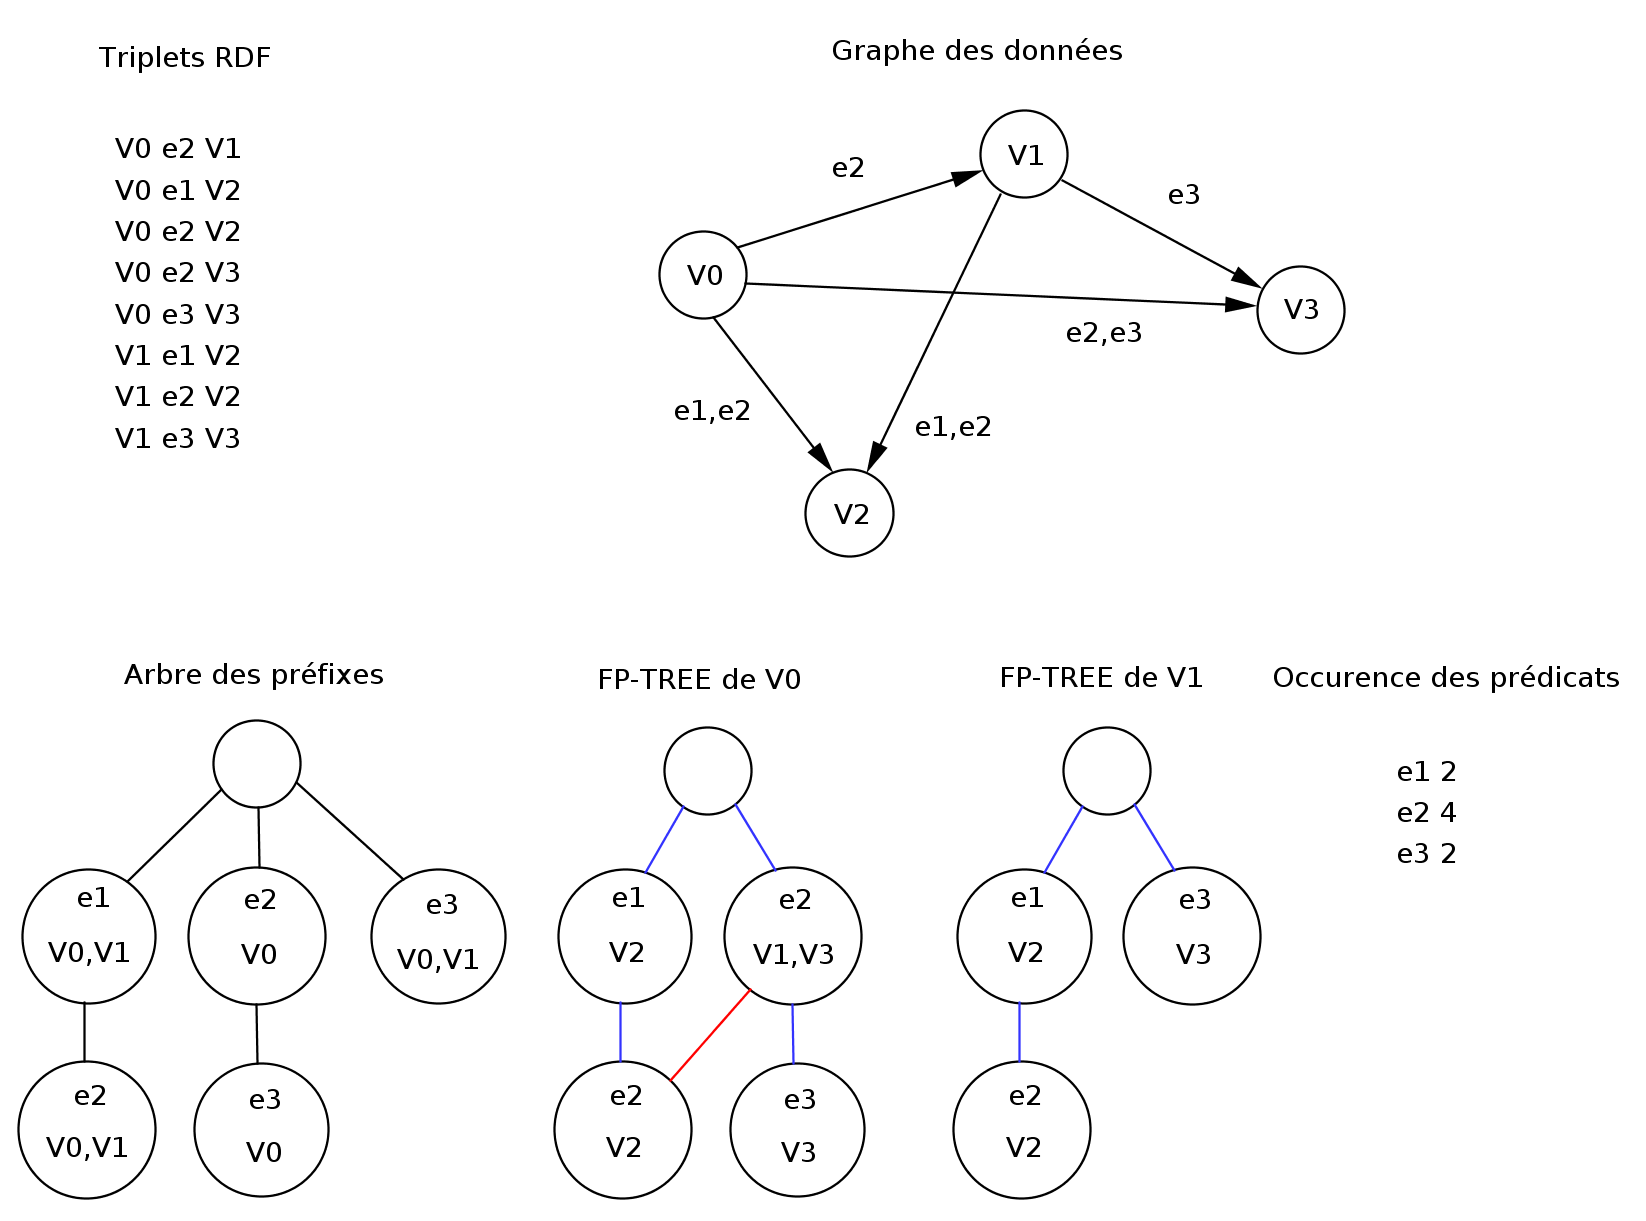
\includegraphics[scale=0.7]{images/import.png}

\end{frame}

\subsection[Requete étoile]{Requete étoile}

\begin{frame}{Exemple de résolution}
  \framesubtitle{Requete étoile}

  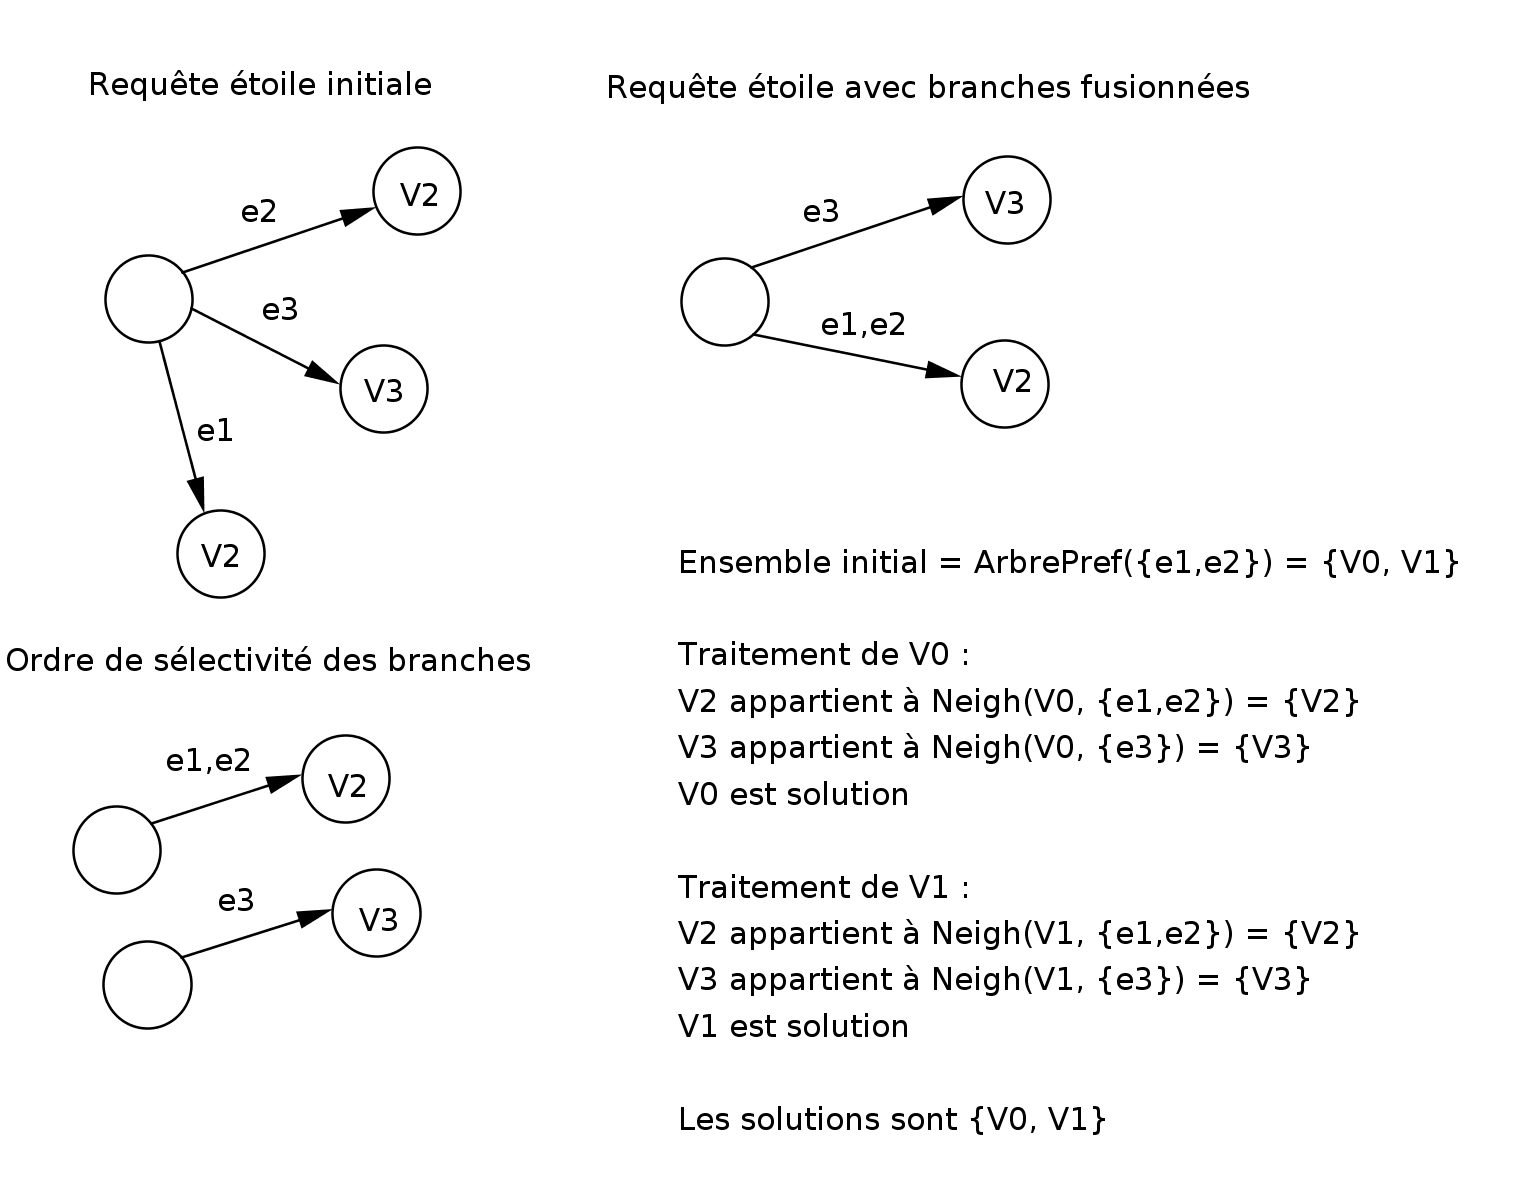
\includegraphics[scale=0.7]{images/query.png}

\end{frame}

\section[Tests]{Tests}

\subsection[Technique d'évaluation]{Technique d'évaluation}
%\begin{comment}

\begin{frame}{Tests}
  \framesubtitle{Technique d'évaluation}

  Les résultats pour 100.000 triplets.
\begin{table}
  \centering
  \resizebox{\columnwidth}{!}{
    \begin{tabular}{|>{\centering\arraybackslash}p{3cm}||>{\centering\arraybackslash}p{2cm}|>{\centering\arraybackslash}p{2cm}|>{\centering\arraybackslash}p{2cm}|>{\centering\arraybackslash}p{2cm}|>{\centering\arraybackslash}p{2cm}|}
      \hline
      \textbf{Système} & \textbf{Temps 1 "Cold"} & \textbf{Temps 2 "Warm"} & \textbf{Temps 3 "Warm"} & \textbf{Temps 4 "Warm"} & \textbf{Temps 5 "Warm"} \\
      \hline
      Notre système & $1.5016 ms$ & $1.4775 ms$ & $1.3883 ms$  & $1.3558 ms$ & $1.3866 ms$\\
      \hline
      Jena& $1.0892 ms$ & $0.9892 ms$ & $1.1584 ms$  & $1.0261 ms$ & $0.97 ms$ \\
      \hline
      Système de Florient Dieu & $0.6388ms$ & $0.5578ms$ &  $0.5476ms$ & $0.4967ms$  & $0.5459ms$ \\
      \hline
    \end{tabular}
}
\end{table}
 
Les résultats pour 500.000 triplets.
\begin{table}
  \centering
  \resizebox{\columnwidth}{!}{
    \begin{tabular}{|>{\centering\arraybackslash}p{3cm}||>{\centering\arraybackslash}p{2cm}|>{\centering\arraybackslash}p{2cm}|>{\centering\arraybackslash}p{2cm}|>{\centering\arraybackslash}p{2cm}|>{\centering\arraybackslash}p{2cm}|}
      \hline
      \textbf{Système} & \textbf{Temps 1 "Cold"} & \textbf{Temps 2 "Warm"} & \textbf{Temps 3 "Warm"} & \textbf{Temps 4 "Warm"} & \textbf{Temps 5 "Warm"} \\
      \hline
      Notre système & $5.9758 ms$ & $5.9366 ms$ & $5.8858 ms$  & $5.8691 ms$ & $5.8875 ms$\\
      \hline
      Jena& $1.8723 ms$ & $1.65 ms$ & $1.4592 ms$  & $1.7138 ms$ & $1.5723 ms$ \\
      \hline
      Système de Florient Dieu & $1.7689ms$ & $1.7381ms$ & $1.6690ms$ & $1.6072ms$ & $1.6061ms$  \\
      \hline
    \end{tabular}
}
\end{table}

\end{frame}

%\end{comment}

\subsection[Temps d'import des données]{Temps d'import des données}

\begin{frame}{Tests}
  \framesubtitle{Temps d'import des données}

  \begin{center}
    Temps d'import des données de notre système, de celui de jena et de celui de Florient Dieu selon 4 types de configuration.
  \end{center}
  \begin{figure}[h]
    \centering
    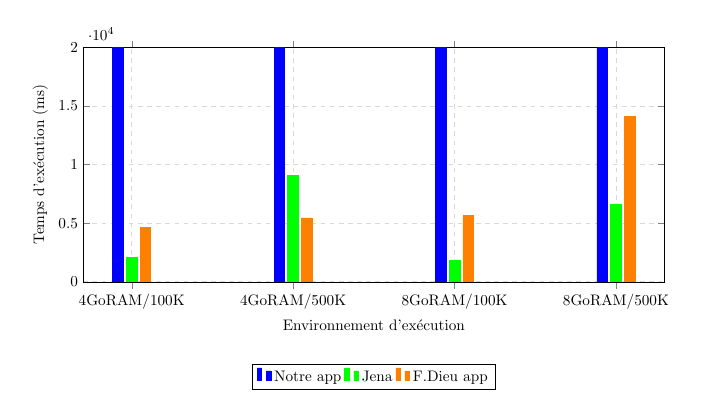
\begin{tikzpicture}[scale=0.55]
      \begin{axis}[
          grid=major,
          width=15cm, height=7cm,
          grid style={dashed,gray!30},
          xlabel=Environnement d'exécution,
          ylabel=Temps d'exécution (ms),
          legend style={at={(0.5,-0.35)},anchor=north,legend columns=-1},
          log ticks with fixed point,
          symbolic x coords={4GoRAM/100K, 4GoRAM/500K, 8GoRAM/100K, 8GoRAM/500K},
          xtick=data,
          ybar,
          ymax=20000,
          bar width=7pt
        ]      
        \addplot[blue,fill] plot coordinates {(4GoRAM/100K, 100000) (4GoRAM/500K,100000) (8GoRAM/100K,258107) (8GoRAM/500K,100000)};
        \addplot[green,fill] plot coordinates {(4GoRAM/100K,2082) (4GoRAM/500K,9097) (8GoRAM/100K,1791) (8GoRAM/500K,6639)};
        \addplot[orange,fill] plot coordinates {(4GoRAM/100K,4628) (4GoRAM/500K,5450) (8GoRAM/100K,5641) (8GoRAM/500K,14078)};
        \legend{Notre app , Jena , F.Dieu app}
      \end{axis}
    \end{tikzpicture}
  \end{figure}
  \begin{center}
    \color{blue} Moyenne arithmétique de 3 temps sur 5
  \end{center}

\end{frame}

\subsection[Temps d'éxécution des requetes]{Temps d'éxécution des requetes}

\begin{frame}{Tests}
  \framesubtitle{Temps d'éxécution des requetes}

  \begin{center}
    Temps d'éxécution des 1200 requetes de notre système, de celui de jena et de celui de Florient Dieu selon 4 types de configuration.
  \end{center}
  \begin{figure}[h]
    \centering
    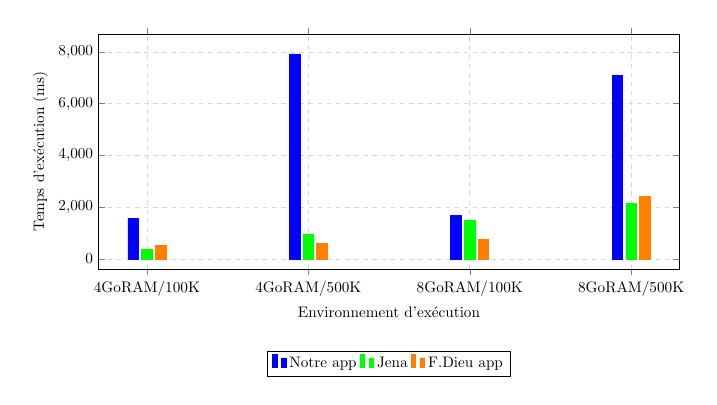
\begin{tikzpicture}[scale=0.55]
      \begin{axis}[
          grid=major,
          width=15cm, height=7cm,
          grid style={dashed,gray!30},
          xlabel=Environnement d'exécution,
          ylabel=Temps d'exécution (ms),
          legend style={at={(0.5,-0.35)},anchor=north,legend columns=-1},
          log ticks with fixed point,
          symbolic x coords={4GoRAM/100K, 4GoRAM/500K, 8GoRAM/100K, 8GoRAM/500K},
          xtick=data,
          ybar,
          bar width=7pt
        ]      
        \addplot[blue,fill] plot coordinates {(4GoRAM/100K,1569) (4GoRAM/500K,7922) (8GoRAM/100K,1669) (8GoRAM/500K,7076)};
        \addplot[green,fill] plot coordinates {(4GoRAM/100K,363) (4GoRAM/500K,959) (8GoRAM/100K,1487) (8GoRAM/500K,2143)};
        \addplot[orange,fill] plot coordinates {(4GoRAM/100K,527) (4GoRAM/500K,583) (8GoRAM/100K,736) (8GoRAM/500K,2416)};
        \legend{Notre app , Jena , F.Dieu app}
      \end{axis}
    \end{tikzpicture}
  \end{figure}
  \begin{center}
    \color{blue} Moyenne arithmétique de 3 temps sur 5
  \end{center}

\end{frame}


\section[Conclusion]{Conclusion}

\begin{frame}{Conclusion}
  \begin{itemize}
  \item Tentative d’optimisation de l’approche
  \item Résultats en dessous des attentes
  \item Ouverture : Pourquoi de tels résultats
  \end{itemize}
\end{frame}

\end{document}
